\chapter{Fundamentação Teórica}
\label{cap:fundamentacao}

Este capítulo apresenta os conceitos de Sistemas Distribuídos, \acrfull{soa} Microsserviços, \acrfull{ddd} e Arquitetura Hexagonal.

\section{Sistema Distribuído} 
\label{section:sistemas_distribuidos}

Um sistema distribuído é um conjunto de componentes independentes entre si que se apresenta aos seus usuários de maneira transparente como um sistema único \cite{tanenbaum2010sistemas}. São sistemas compostos por diversas partes cooperantes, que são executadas geralmente em processos diferentes interconectados por rede a fim de realizar alguma tarefa. 

Diferentemente de sistemas monolíticos, nos quais todos os módulos estão interligados em uma única unidade, os sistemas distribuídos dividem o processamento entre as partes. Essa abordagem traz vantagens significativas, como a possibilidade de escalabilidade horizontal e maior flexibilidade para atualizar e substituir componentes individuais sem afetar o sistema como um todo e o compartilhamento de recursos.

Um dos principais desafios desse tipo de sistema é a concorrência e coordenação entre os componentes. Nessa abordagem, vários componentes podem estar operando simultaneamente e em diferentes locais físicos, o que gera problemas de concorrência, onde múltiplos processos tentam acessar os mesmos recursos compartilhados ou dados simultaneamente. Por esse motivo, torna-se essencial a coordenação entre esses processos para evitar conflitos e garantir a consistência dos dados.

\subsection{\english{\acrfull{soa}}} 
A arquitetura orientada a serviços ou \acrfull{soa} é estilo arquitetural no qual um sistema é dividido em componentes de software chamados de serviços, responsáveis por satisfazer uma necessidade de negócio específica.

As políticas, práticas e \english{frameworks} que permitem que a funcionalidade da aplicação seja fornecida e consumida como conjuntos de serviços publicados em uma granularidade relevante para o consumidor do serviço. Os serviços podem ser invocados, publicados e descobertos, e são abstraídos da implementação usando uma única forma de interface baseada em padrões \cite{understandingSOA}.

As principais vantagens da \acrshort{soa} são: reusabilidade dos serviços, simplicidade de manutenção, facilidade de escalar os serviços, maior disponibilidade do sistema e possibilidade de utilização de diferentes tecnologias nos serviços.

Porém, essa arquitetura possui uma maior complexidade para \english{design}, desenvolvimento, teste e implantação. Além desses fatores, é importante ressaltar um nível maior de dificuldade para depurar erros e encontrar profissionais qualificados para atuar nessa área.

\section{Microsserviços} 
A \acrfull{ams} é um subtipo da \acrshort{soa}. No entanto, trata-se de uma subcategoria que orienta como as fronteiras entre os serviços devem ser traçadas e que possui como ponto central a independência de implantação entre os serviços \cite{buildingMicroservices}.

Esse estilo arquitetural foca na criação de um sistema robusto, escalável e de fácil manutenção, desenvolvido através da composição de serviços pequenos, flexíveis e que resolvam uma necessidade negócio específica \cite{buildingMicroservices}. Além disso, cada microsserviço deve possuir sua própria base de dados. A troca de informações entre os componentes deve ser realizada através das interfaces fornecidas.

A implantação de um sistema com a utilização de microsserviços aumenta a resiliência geral do sistema, visto que possui melhor isolamento de falhas. Caso ocorra um mal-funcionamento em algum componente, somente uma parte das funcionalidades ficará indisponível. Tratando-se de um monólito, por outro lado, grande parte ou a totalidade dos recursos são afetados, pois todo o sistema é acoplado em uma única unidade.

Cada serviço na \acrshort{ams} pode ser escalado de maneira independente de outros serviços utilizando, por exemplo, escalonamento horizontal ou vertical \cite{richardson2018microservices}. Ademais, para cada serviço pode ser selecionado o \english{hardware} mais adequado para seu tipo de processamento. Dessa forma, uma parte do sistema que requer maior utilização da CPU pode ser implantada em uma infraestrutura diferente de outra secção que necessita realizar mais operações de entrada e saída.

Outro benefício dessa arquitetura é o fato de cada serviço ser relativamente pequeno, sendo, assim, de fácil compreensão por todos que trabalham na base de código. Adicionalmente, um serviço pequeno possibilita um bom desempenho da \acrshort{ide} e também pode ser executado localmente de maneira rápida. Esses fatores contribuem para um aumento de produtividade da equipe \cite{richardson2018microservices}.

Por outro lado, com um sistema composto de múltiplos componentes, torna possível a utilização de diferentes tecnologias dentro da cada serviço. Dessa forma, a ferramenta mais apropriada para resolver a necessidade específica do serviço pode ser selecionada, eliminando a obrigatoriedade de escolher uma única tecnologia para todo o sistema \cite{buildingMicroservices}.

\subsection{Comunicação entre microsserviços}
Quando um sistema é composto por um único monólito, a comunicação entre os diferentes módulos é simplificada, pois se trata de um único processo a nível do sistema operacional e, portanto, compartilha a área da memória principal. No entanto, microsserviços são implantados em diferentes processos(usualmente em diferentes computadores), assim se faz necessária a utilização de algum mecanismo de comunicação entre processos, também conhecido como \acrfull{ipc}.

Existe no mercado uma série de tecnologias, protocolos e ferramentas que viabilizam a comunicação entre microsserviços. Porém, antes de selecionar o mecanismo de \acrshort{ipc}, é importante compreender os estilos de interações entre sistemas \cite{richardson2018microservices}. Essa abordagem coloca foco nos requisitos da aplicação, no lugar de detalhes de um mecanismo específico.

Os modos de interação entre um cliente e um serviço podem ser classificados em duas dimensões: a quantidade de serviços que processam a requisição e a sincronicidade. No que diz respeito à primeira dimensão, existem duas opções: \textbf{"um para um"}, em que cada requisição é processada por um único serviço; e \textbf{"um para muitos"}, em que cada requisição pode ser processada por vários serviços. Por outro lado, a comunicação pode ser \textbf{síncrona}, onde o cliente espera uma resposta imediata e geralmente aguarda essa resposta para continuar seu processamento; ou \textbf{assíncrona}, onde o cliente envia a requisição e continua seu processamento sem esperar por uma resposta \cite{richardson2018microservices}.

\begin{quadro}[H]
\centering
\caption{Estilos de comunicação entre microsserviços}
\setlength{\tabcolsep}{0.8em} % for the horizontal padding
\renewcommand{\arraystretch}{1.5}% for the vertical padding
\begin{tabular}{p{1.5in}p{1.5in}p{1.5in}}
\hline

%row no:1
\multicolumn{1}{|p{1.5in}}{\textbf{}} & 
\multicolumn{1}{|p{1.5in}}{\textbf{Um para um}} & 
\multicolumn{1}{|p{1.5in}|}{\textbf{Um para muitos}} \\
\hhline{---}

%row no:2
\multicolumn{1}{|p{1.5in}}{\textbf{Síncrona}} & 
\multicolumn{1}{|p{1.5in}}{\english{Request/Response}} & 
\multicolumn{1}{|p{1.5in}|}{-} \\
\hhline{---}

%row no:3
\multicolumn{1}{|p{1.5in}}{\textbf{Assíncrona}} & 
\multicolumn{1}{|p{1.5in}}{\english{Asynchronous request/response} e \english{One-way notifications}} & 
\multicolumn{1}{|p{1.5in}|}{\english{Publish/subscribe} \english{Publish/async responses}} \\
\hhline{---}
\end{tabular}
\label{quad:estilos_comunicacao}
\fonte{\citeonline{richardson2018microservices}.}
\end{quadro}

No \autoref{quad:estilos_comunicacao}, observam-se alguns estilos de comunicação categorizados pelas dimensões anteriormente mencionadas. No \autoref{quad:padroes_um_para_um} são apresentados os diferentes tipos de comunicação \textbf{"um para um"}:

\begin{quadro}[H]
\centering
\caption{Padrões de comunicação do tipo \textbf{"um para um"}}
\setlength{\tabcolsep}{0.8em} % for the horizontal padding
\renewcommand{\arraystretch}{1.5}% for the vertical padding
\begin{tabular}{|p{1.2in}|p{3.5in}|}
\hline

\textbf{Nome} & \textbf{Descrição} \\ \hline
\english{Request/Response} & O serviço cliente realiza uma requisição a outro serviço e espera(geralmente bloqueando sua execução) por uma resposta. \\ \hline
\english{Asynchronous request/response} & O serviço cliente envia uma solicitação a um serviço, que responde de forma assíncrona. O cliente não fica bloqueado enquanto espera, pois o serviço pode não enviar a resposta por um longo período.\\ \hline
\english{One-way notifications} & O serviço cliente envia uma requisição, mas não espera nenhum tipo de resposta do serviço que processará a requisição. \\ \hline

\end{tabular}
\label{quad:padroes_um_para_um}
\fonte{\citeonline{richardson2018microservices}.}
\end{quadro}

Frequentemente, em ambientes de sistemas distribuídos, há a necessidade de vários serviços consumirem uma mensagem produzida por um determinado serviço. Nesse sentido, no \autoref{quad:padroes_um_para_muitos} são listadas algumas opções de padrões para realizar comunicações do tipo \textbf{"um para muitos"}:

\begin{quadro}[H]
\centering
\caption{Padrões de comunicação do tipo \textbf{"um para muitos"}}
\setlength{\tabcolsep}{0.8em} % for the horizontal padding
\renewcommand{\arraystretch}{1.5}% for the vertical padding
\begin{tabular}{|p{1.2in}|p{3.5in}|}
\hline

\textbf{Nome} & \textbf{Descrição} \\ \hline
\english{Publish/Subscribe} & Um cliente publica uma mensagem, que é consumida por zero ou mais serviços.. \\ \hline
\english{Publish/async responses} & Um cliente publica uma mensagem contendo uma requisição e espera por um determinado período por respostas. \\ \hline

\end{tabular}
\label{quad:padroes_um_para_muitos}
\fonte{\citeonline{richardson2018microservices}.}
\end{quadro}

\subsection{Estratégias para delimitação de microsserviços}
Uma decisão de grande impacto no projeto de sistema que utilize a \acrshort{ams} é o escopo de cada serviço. Em outras palavras, que funcionalidades serão parte de um determinado serviço e quais serão delegadas a outro componente.

\citeonline{buildingMicroservices} argumenta que a possibilidade de alterar um microsserviço de maneira isolada é fundamental para essa arquitetura. Além disso, \acrshort{ams} é apenas outra forma de decomposição modular, afirma o autor. Assim, os conceitos de \english{information hiding}, coesão e acoplamento podem ser aplicados nesse contexto para criar as delimitações eficientes entre os serviços.

\english{Information hiding} é uma abordagem para desenvolvimentos de módulos, na qual se busca esconder o máximo de detalhes possíveis detrás da interface de um módulo \cite{buildingMicroservices}. Dessa forma, os benefícios esperados com a construção de módulos de alta qualidade são:
\begin{itemize}
    \item \textbf{Tempo de desenvolvimento aprimorado:} com a possibilidade de módulos serem construídos de forma independente, o desenvolvimento pode ser realizado de maneira paralela.
    \item \textbf{Compreensibilidade:} cada módulo pode ser entendido de maneira isolado. Assim, se torna mais fácil compreender o que o sistema como um todo faz.
    \item \textbf{Flexibilidade:} módulos podem ser modificados de maneira independente, possibilitando, dessa forma, alterações em uma parte do sistema sem a necessidade de alterações em outros módulos.
\end{itemize}
\cite{Parnas2012}.

Coesão diz respeito à medida que os elementos dentro de um módulo estão organicamente relacionados entre si \cite{Yourdon1979}. Outra definição possível é código que, alterado conjuntamente, deve estar localizado no mesmo lugar \cite{buildingMicroservices}. No contexto da \acrshort{ams}, a adição ou atualização de funcionalidades deve, idealmente, envolver um único serviço. Dessa forma, é possível disponibilizar novos recursos aos usuários de maneira mais ágil \cite{buildingMicroservices}. Por esse motivo, buscar alta coesão é importante no momento da definição do escopo de cada serviço. O objetivo principal é evitar que sejam necessárias alterações em múltiplos serviços no desenvolvimento de funcionalidades para o sistema.

Quando serviços são fracamente acoplados, uma alteração em um serviço não requer alteração no outro \cite{buildingMicroservices}. A grande vantagem da \acrshort{ams} é a possibilidade de realizar mudanças em partes do sistema de maneira isolada. Nesse sentido, a projeção de serviços com alta coesão e fraco acoplamento é essencial para que os objetivos da utilização dessa tecnologia sejam atingidos. Nem todo acoplamento é necessariamente maléfico. De fato, algum nível de acoplamento entre os serviços é inevitável. Além disso, há diferentes tipos de acoplamento listados no \autoref{quad:tipos_acoplamento}.

\begin{quadro}[H]
\centering
\caption{Tipos de acoplamento}
\setlength{\tabcolsep}{0.8em} % for the horizontal padding
\renewcommand{\arraystretch}{1.5}% for the vertical padding
\begin{tabular}{|p{1.2in}|p{3.5in}|}
\hline

\textbf{Tipo} & \textbf{Descrição} \\ \hline
\english{Domain Coupling} & Descreve uma situação em que um microsserviço necessita interagir com outro serviço para fazer uso de sua(s) funcionalidade(s). Na \acrshort{ams}, esse tipo de iteração é quase inevitável. No entanto, é necessário que cada serviço exponha o mínimo de detalhes possível (\english{information hiding}) para não gerar um nível de acoplamento muito alto. \\ \hline
\english{Pass-Through Coupling} & Acontece quando um microsserviço envia dados a outro serviço somente porque essas informações são necessárias por um terceiro serviço. Trata-se de um dos tipos de acoplamento mais problemáticos, pois implica que o cliente da primeira requisição conheça tanto o serviço que inicialmente recebe a requisição, quanto o que irá, de fato, utilizar os dados. \\ \hline
\english{Common Coupling} & Ocorre quando dois ou mais microsserviços compartilham o mesmo conjunto de dados. O exemplo mais comum desse tipo de acoplamento é a utilização de uma base de dados compartilhada. O principal problema dessa abordagem é o fato de modificações ou falhas na base de dados compartilhadas afetar mais de um serviço. \\ \hline
\english{Content Coupling} & Descreve uma situação em que o serviço acessa e modifica estados internos de outro serviço. É semelhante ao \english{Common coupling}, porém nesse caso as linhas de responsabilidades de cada serviço se tornam confusas. Assim, desenvolvedores encontram grandes dificuldades para realizar alterações. \\ \hline

\end{tabular}
\label{quad:tipos_acoplamento}
\fonte{\citeonline{buildingMicroservices}.}
\end{quadro}

Visando a construção de serviços com alta coesão e baixo acoplamento, portanto estáveis, os conceitos de \acrshort{ddd} podem ser utilizados. Uma abordagem interessante e comumente aplicada é mapear um \nameref{section:bounded_context} para cada serviço \cite{buildingMicroservices}. Como os \hyperref[section:bounded_context]{Bounded Contexts} representam uma parte do domínio onde um modelo se aplica, eles permitem que microsserviços sejam modelados ao redor de uma secção coesa e completamente funcional que ofereça funcionalidades de negócio. Outra opção para modelagem de microsserviços é mapear cada \nameref{section:aggregate} para um serviço. Essa estratégia oferece um nível de granularidade menor que um \nameref{section:bounded_context}, visto que este geralmente engloba múltiplos \nameref{section:aggregate}s. No entanto, \citeonline{buildingMicroservices} sugere recorrer primeiro a delimitações maiores na construção de microsserviços, englobando um (ou até mais) \nameref{section:bounded_context}. Dessa forma, caso a equipe sinta necessidade de subdividir o serviço, poderá fazê-lo sem complicações.

Apesar de \acrfull{ddd} ser uma excelente maneira de delimitar microsserviços, não é a única técnica disponível \cite{buildingMicroservices}. São listadas a seguir algumas alternativas frequentemente utilizadas:
\begin{itemize}
    \item \textbf{Volatilidade:} decomposição baseada em volatilidade refere-se a uma abordagem, na qual partes do sistema que são frequentemente alteradas são extraídas em seus próprios serviços, de forma que possam ser trabalhadas de maneira mais efetiva. Essa estratégia por ser útil em organizações com ritmo de mudanças acelerado. No entanto, se o objetivo da utilização da \acrshort{ams} é a possibilidade de escalar partes do sistema de maneira independente, decomposição baseada em volatilidade não atingirá a meta.
    \item \textbf{Dados:} a natureza das informações que necessitam ser armazenadas pode direcionar a estratégia de decomposição. Por exemplo, é muito usual restringir quais microsserviços podem acessar informações de identificação pessoal para cumprir com legislações como a Lei Geral de Proteção de Dados Pessoais.
    \item \textbf{Tecnologia:} A necessidade de se utilizar diferentes tecnologias também pode ser um fator a se considerar na definição do escopo de um microsserviço. Se há a necessidade, por exemplo, de alto desempenho em uma parte do sistema que demande a utilização de uma linguagem de programação diferente, este pode ser um ponto importante para delimitação do serviço.
\end{itemize}
\cite{buildingMicroservices}.

É importante mencionar que essas opções não são mutualmente exclusivas. Em um sistema real, provavelmente uma mistura de estratégias necessitará ser aplicada para satisfazer os requisitos funcionais e não-funcionais.

\subsection{Desafios na implementação de microsserviços}
Certamente, não há nenhuma tecnologia que não possua limitações. Isso não é diferente com a \acrlong{ams} \cite{richardson2018microservices}. 

Primeiramente, como microsserviços baseiam-se no conceito de \nameref{section:sistemas_distribuidos}, uma série de novos problemas estão presentes nessa arquitetura. Como os serviços necessitam utilizar algum mecanismo de \acrshort{ipc}, há um grande aumento na complexidade do ciclo de desenvolvimento como um todo. \acrshort{ide}s e outras ferramentas de desenvolvimento possuem maior foco no desenvolvimento de aplicações monolíticas. Adicionalmente, escrever testes automatizados envolvendo múltiplos serviços é uma tarefa complexa. Além disso, a \acrshort{ams} introduz dificuldades significantes de operação, como necessidade de alto nível de automação e ferramentas de monitoramento avançadas. Assim, uma equipe técnica altamente qualificada se torna necessária, podendo inclusive ser útil a contratação de consultorias especializadas nessa tecnologia \cite{richardson2018microservices}.

Por outro lado, a \acrfull{ams} engloba desafios para manter a consistência dos dados. Enquanto em um sistema monolítico, dados são usualmente armazenados em uma única base de dados relacional, que oferece suporte a transações \acrshort{acid}, em um sistema distribuído, no qual múltiplos banco de dados - possivelmente de tipos e fornecedores diferentes - são empregados, esse tipo de segurança não pode ser atingido facilmente \cite{buildingMicroservices}. Transações distribuídas ou \english{Sagas} podem ser aplicadas para reduzir problemas de consistência, no entanto, essas técnicas adicionam grande complexidade ao sistema \cite{buildingMicroservices}.

\section{\english{Domain-Driven Design (DDD)}} 
\english{\acrfull{ddd}} é uma abordagem para o desenvolvimento de software focada na construção de um modelo de domínio que representa de maneira sofisticada os processos e regras de negócio do sistema em questão \cite{dddFowler}. \acrshort{ddd} é muito efetivo para desenvolver sistemas com regras de negócio complexas, que possuem, por exemplo, diversos atores, entidades e validações. A \acrfull{poo} é geralmente empregada para a implementação do modelo de domínio, visto que possui uma série de recursos que facilitam a modelagem de objetos do mundo real \cite{evans2004ddd}.

Um ponto central da metodologia \acrshort{ddd} no desenvolvimento de softwares complexos, é a utilização de uma linguagem ubíqua que insere terminologia e jargões do domínio em componentes de software como atributos, métodos, classes, interfaces e pacotes \cite{dddFowler}. Assim, tanto especialistas de negócio quanto desenvolvedores e projetistas compartilham um vocabulário comum que facilita na comunicação e reduz a necessidade de realizar o mapeamento entre termos técnicos e termos do domínio. Além disso, a estrutura de sistema passa a representar a estrutura do negócio, tornando-se, assim, mais fácil de ser compreendida e modificada.

O nome dessa estrategia vem de um livro publicado em \citeyear{evans2004ddd} por Eric Evans que descreve a abordagem, uma série de conceitos e um catálogo de  padrões comumente utilizados para resolução de problemas de modelagem de domínios. Os mais relevantes dentre estes são descritos a seguir.

\subsection{Modelo e Domínio}
Os conceitos de modelo e domínio, no contexto da engenharia de software, são fundamentais para o entendimento do \acrshort{ddd}. Modelo é uma simplificação, uma interpretação da realidade que abstrai os aspectos relevantes para resolver o problema em questão e ignora detalhes superficiais \cite{evans2004ddd}. Da mesma forma, todo sistema computacional está relacionado a alguma atividade ou interesse do usuário final. Assim, a área para qual o usuário utiliza o sistema é domínio do software \cite{evans2004ddd}. Alguns exemplos de domínios comuns são: financeiro, médico, logística e \english{marketplace}.

\subsection{Entidade}
No contexto da \acrfull{poo}, muitos objetos não são fundamentalmente definidos por seus atributos, mas por um fio de continuidade e identidade \cite{evans2004ddd}. Eles podem ter distintas representações como, por exemplo, em memória ou em um banco de dados. No entanto, eles necessitam ser distinguíveis mesmo se todas suas propriedades forem iguais. Em um domínio financeiro, por exemplo, uma transação composta por valor, data e usuário necessita ser diferenciável de outra transação com as mesmas características. Por outro lado, para uma classe fictícia chamada \english{Money} composta por valor e moeda, dois objetos com os mesmos atributos podem ser geralmente considerados iguais, sem gerar corrupções de dados ou impactos para os usuários finais do sistema. Em resumo, quando um objeto definido principalmente por sua identidade, ele é chamado de Entidade \cite{evans2004ddd}.

\subsection{\english{\acrfull{vo}}}
Muitos objetos não possuem identidade conceitual, sendo somente utilizados para descrever características de outro objeto. São objetos que descrevem coisas, classificados como \acrfull{vo} \cite{evans2004ddd}. Para um sistema de uma loja de roupas, por exemplo, um objeto que representa cor de cada peça formado pelas propriedades \english{red}, \english{green} e \english{blue}, não possui identidade. Não necessita ser diferenciável de outro objeto com as mesmas propriedades. Este objeto somente descreve uma característica de uma peça de roupa. É importante ressaltar, porém, que a diferenciação entre Entidade e \english{\acrlong{vo}} depende do contexto do software. Para um sistema de software de computação gráfica, a cor é um conceito chave no sistema e pode possuir identidade.

Pode-se pensar que é mais vantajoso sempre projetar os objetos do sistema como Entidade, pois adicionaria identidade, facilitaria o rastreamento de mudanças e agregaria mais recursos ao objeto. No entanto, a adição de identidade para objetos que não necessitam desta classificação pode prejudicar o desempenho do sistema, adicionar mais esforço de análise e aumentar a complexidade do modelo de domínio \cite{evans2004ddd}. Por esse motivo, recomenda-se a utilização de \acrshort{vo} sempre que for possível, pois se tratam de objetos mais fáceis de gerenciar.

\subsection{Serviço}
Em muitos casos, há operações importantes no modelo que não pertencem conceitualmente a nenhuma Entidade ou \acrshort{vo}. Dessa forma, surge o conceito de Serviço: uma operação fornecida como uma interface autônoma no modelo, sem encapsular estado como outros tipos de objeto \cite{evans2004ddd}.

Um erro comum é a abusar da utilização de Serviços, desistindo de encontrar o objeto apropriado para uma operação de domínio. Da mesma forma, a inserção de um método que não está alinhado com a definição do objeto resulta na perda de coesão desse objeto, tornando-o mais difícil de compreender e refatorar \cite{evans2004ddd}. Considerando esses pontos, um serviço deve ser utilizado quando um processo ou transformação relevante no modelo de domínio não faz parte da responsabilidade natural de uma Entidade ou \acrshort{vo}.

Além disso, \citeonline{evans2004ddd} destaca três características de um bom Serviço:
\begin{itemize}
    \item A operação não possui estado (\english{stateless}).
    \item A interface é defina em termos de outros elementos do modelo de domínio.
    \item A operação se relaciona a um conceito do modelo que não é parte natural de uma Entidade ou \acrshort{vo}.
\end{itemize}

\subsection{\textit{Aggregate}}
\label{section:aggregate}
Um \english{Aggregate} é um conjunto de objetos associados, tratados como uma única unidade para o proposito de alterações de dados \cite{evans2004ddd}. Em um sistema de grande porte, é difícil garantir a consistência de alterações em objetos com relacionamentos complexos. As invariantes que precisam ser mantidas geralmente envolvem um grupo de objetos intimamente associados, ao invés de objetos isolados. Assim, o padrão \english{Aggregate} propõe delimitações definidas e restrições de acesso visando o melhor tratamento das associações entre objetos.

Cada \english{Aggregate} possui uma raiz e uma delimitação, que define o que está dentro do \english{Aggregate} \cite{evans2004ddd}. A raiz é a única entidade global - que possui identidade em todo o sistema - contida dentro do \english{Aggregate}, também conhecida como \english{Aggregate root} \cite{evans2004ddd}. Objetos fora da delimitação do \english{Aggregate} só podem possuir referências a raiz e não a outros objetos dentro do \english{Aggregate}. Excluindo a raiz, outras entidades somente possuem identidade local, necessitando somente ser distinguíveis dentro dos limites do \english{Aggregate}, visto que nenhum objeto de fora consegue obtê-las desassociadas da entidade raiz \cite{evans2004ddd}.

\subsection{\acrfull{bc}}
\label{section:bounded_context}
Em grandes projetos, muitos modelos coexistem em diferentes contextos. Quando a base de código, no entanto, combina diferentes modelos sem que haja uma separação clara, o \english{software} se torna defeituoso, frágil e difícil de ser compreendido \cite{evans2004ddd}. Assim, é necessário especificar em qual o contexto um determinado modelo está sendo aplicado.  Assim, um \english{\acrfull{bc}} delimita a aplicabilidade de um modelo, de tal forma que os membros da equipe tenham um entendimento claro do que precisa ser consistente e a relação do modelo com outros contextos. Um \acrshort{bc} engloba tanto componentes de modelo como \english{Aggregates}, Entidades, \english{\acrlong{vo}}s e Serviços, quanto detalhes técnicos como persistência. É uma parte completa e funcional de software sob responsabilidade de uma única equipe.

Por exemplo, um \english{software} para um \english{e-commerce} possui um módulo que lida com pedidos, em que cada pedido contém um ou mais produtos. Da mesma forma, outra equipe é responsável por um módulo de realiza o gerenciamento de produtos em estoque. O conceito de um produto para um sistema de pedidos é distinto de uma aplicação de estoque. Enquanto este pode ter um enfoque no armazém, na categoria e no estoque do produto, aquele está mais preocupado com o preço, nome e disponibilidade. Assim, ao tratar esses dois conceitos da maneira igual, confusões e defeitos são gerados.

\section{Arquitetura Hexagonal} 
\label{section:hexagonal}
A arquitetura hexagonal, também conhecida como \english{Ports and Adapters}, possui como objetivo isolar regras de negócio de agentes externos \cite{cockburn2005}. Nesse sentido, o que está dentro do hexágono representa o modelo de domínio. Do mesmo modo, componentes de fora representam detalhes de implementação, como persistência, interface de usuário, envio de \english{e-mails}, entre outros. Um ponto crucial nessa arquitetura é a direção das dependências: o que está dentro do hexágono não pode depender do que está fora. Assim, é a garantida a independência e o isolamento de regras de negócio das dependências técnicas.

\begin{figure}[!ht]
    \centering
    \caption{Arquitetura Hexagonal}
    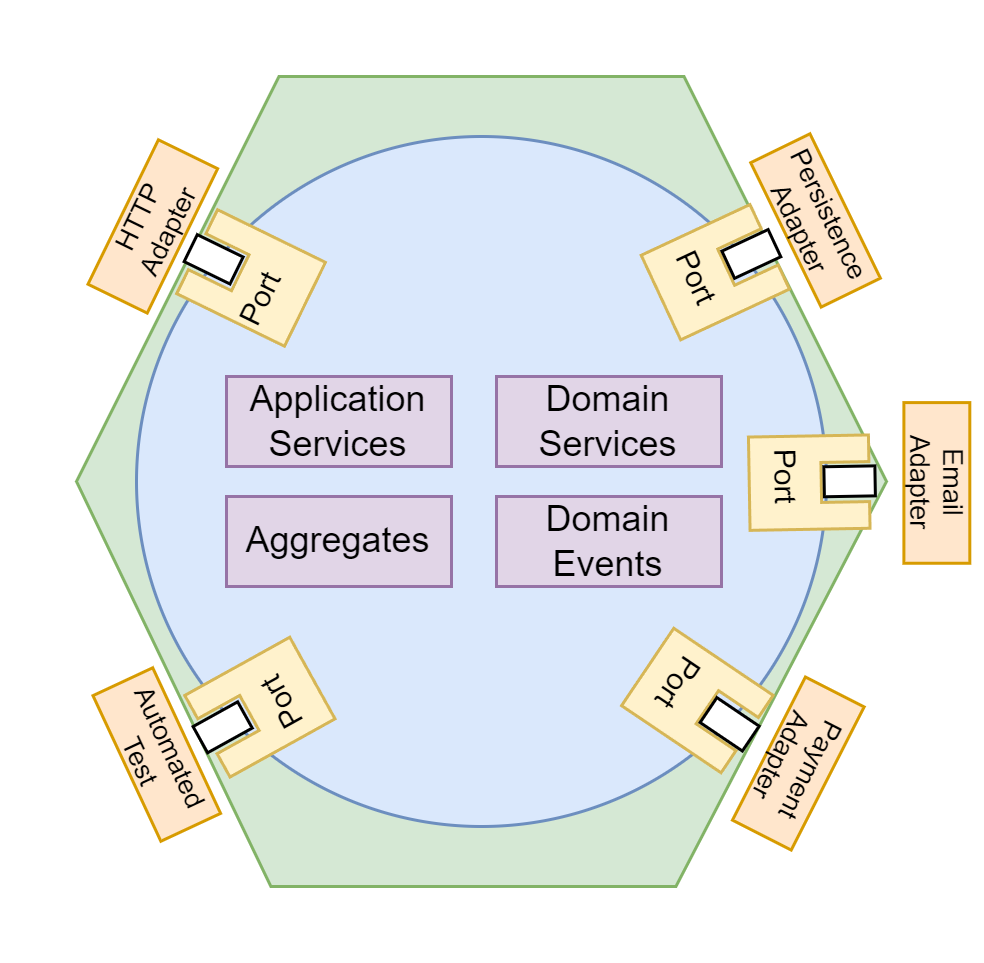
\includegraphics[width=0.75\textwidth]{media/hexagonal_architecture.png}
    \legend{Fonte: o autor}
    \label{fig:arquitetura_hexagonal}
\end{figure}

Na \autoref{fig:arquitetura_hexagonal}, pode-se observar que a injeção de agentes externos, como persistência em um banco de dados, é realizada por meio de portas definidas dentro do núcleo da aplicação. As portas, nessa arquitetura, são geralmente representadas por interfaces em linguagens orientadas a objetos. Então, um adaptador fornece uma implementação de uma tecnologia específica para a porta. Assim, implementações para tecnologias específicas são definidas em função do modelo de domínio.

Outros benefícios importantes, além do isolamento das regras de negócio, são: facilidade de testar o núcleo da aplicação com a utilização de \english{mocks} e \english{stubs}; possibilidade de utilização da mesma aplicação via interfaces de usuário, testes automatizados e \english{batches}.

Enquanto a \acrfull{ams} visa organizar um sistema como um conjunto de serviços independentes, cada um executando uma função específica, a arquitetura hexagonal concentra-se na organização interna de um serviço, propondo uma separação clara entre a lógica de negócios e as implementações técnicas, usando portas e adaptadores. Por outro lado, \acrshort{ddd} apresenta-se como uma excelente abordagem para desenvolvimento do núcleo da aplicação na arquitetura hexagonal. Assim, esses três conceitos: microsserviços, arquitetura hexagonal e \acrshort{ddd} podem ser combinados para o desenvolvimento de sistemas altamente coesos, desacoplados, escaláveis, inteligíveis e sustentáveis.




